\documentclass{article}

\usepackage[utf8]{inputenc}
\usepackage{datetime}
\usepackage{amsthm}
\usepackage{amsmath}
\usepackage{amssymb}
\usepackage{enumitem}
\usepackage[USenglish]{babel}
\usepackage{listings}
\usepackage{graphicx}
\graphicspath{ {images/} }
\usepackage{subcaption}
\usepackage{float}
\usepackage[makeroom]{cancel}
\usepackage{afterpage}
\usepackage{capt-of}
\usepackage{hyperref}

\DeclareMathOperator*{\argmin}{arg\,min}
\DeclareMathOperator*{\argmax}{arg\,max}

\title{ORFE 510 Report}
\author{Zachary Hervieux-Moore}

\newdate{date}{09}{05}{2018}
\date{\displaydate{date}}

\begin{document}

  \maketitle

  \clearpage

  \tableofcontents
  \listoffigures

  \clearpage

  \section{Introduction}

  In October 2015, Google shocked the world by creating a computer program (AlphaGo) that beat a professional at the game of Go. Something that had never been accomplished before. A couple of months later, the team published the algorithm that powered the program \cite{silver_mastering_2016}. Later that year, the team published another paper outlining a new algorithm that was even more powerful than the first and learned the game entirely from self-play and no human knowledge \cite{silver_mastering_2017}. Finally, the team published a follow-up a last month showing the robustness of the algorithm (AlphaZero) by using it to create the best known player in three different games: Go, chess, and shogi \cite{silver_mastering_2017-1}.

  The work done by the Google team was ground breaking and was a big step forward as they seemingly solved the ``curse of dimensionality'' for the game of Go. Go has approximately $2 \times 10^{170}$ legal positions \cite{tromp_sequence_2016}. This is what made the game of Go such a difficult game to solve. Many reinforcement learning algorithms, such as Q-Learning, require the storage of a transition matrix which would be massive for the game of Go. The innovation of AlphaZero is leveraging deep neural networks to somehow compress the state representation. However, there is an issue with the AlphaZero algorithm. Namely, it requires a fairly small action space. In the game of Go, one only has on the order of 361 ($19 \times 19$) moves to consider at each step. Chess and shogi also represent ``simple'' games in this regard as each move only has a small amount of possible actions. With these small action spaces, AlphaZero is able to get away with having to worry about considering each and every possible move. However, if we consider a game like Scrabble, where tiles are randomly drawn at the end of your turn, even performing the same action can lead to millions of different states. It is precisely this deficiency that I've been focusing on and this report will outline my work I've done this past semester.

  The report will be broken down in the following manner. First, I will present the relevant works required to have an understanding of what I'm working on. This will consist of a review bandit theory, Monte Carlo tree search, the AlphaGo and AlphaZero algorithms, and finally the prior art for Scrabble AI. Next, I will present the work I have accomplished thus far. This will mainly consist of the code I have developed for creating a framework such that I can experiment with different versions of the algorithm as well a preliminary resutls. Finally, I will have a section on future work that I hope to work on and other possible interesting avenues of research.

  \clearpage

  \section{Background}

  \subsection{Multi-armed Bandit Theory}
  The following sections are motivated by the multi-armed bandit problem. So we start with the typical problem formulation. Suppose there are $K$ machines that give rewards according to some distribution in $[0,1]$. Then we define the random variable $X_{i,n}$ for $1 \leq i \leq K$ and $n \geq 1$, where $i$ is the index for the $i^{th}$ machine and $n$ is the number of times that machine has been pulled. That is, $X_{i,n}$ is the reward that was received for picking machine $i$ for the $n^{th}$ time. Now, suppose each machine has an unknown expected reward $\mu_j$. Finally, suppose we have a strategy to pick the machines. Define $T_j(n)$ to be the number of times the strategy picks machine $j$ on the $n^{th}$ pull. Then we define regret to be:

  \begin{gather*}
    \mu^*n - \mu_j \sum_{j=1}^K \mathbb{E} [T_j(n)] \quad \text{ where } \mu^* = \max_{i \leq i \leq K} \mu_i
  \end{gather*}

  First let us point out that if one simply pulls the same machine continuously (we call this strategy purely exploitation), the expected regret is linear. This is from the fact that there is a $(K-1)/K$ chance of picking a suboptimal machine. Conversely, if one purely explores, each time picking machine $j$ with probability $1/K$, a similar analysis will yield a linear regret. The question then becomes if there is a strategy that balances exploitation and exploration to achieve sublinear regret. This is indeed the case as presented in \cite{auer_finite-time_2002}. In this work, they present the \textit{upper confidence bound} (UCB) strategy which achieves worst-case regret on the order of $O(\sqrt{K n \log(n)})$. The UCB strategy is simply keeping track of the empirical averages of the rewards from each machine ($\bar{x}_j$) and picking the machine that maximizes

  \begin{gather*}
    \bar{x}_j + \sqrt{\frac{2 \ln n}{n_j}}
  \end{gather*}

  Where $n_j$ is the number of times that machine $j$ has been picked. Using UCB and applying to decision trees was a natural extension. This was done in \cite{kocsis_bandit_2006} to develop a novel rollout-based Monte Carlo planning algorithm. They called this algorithm \textit{UCB applied to trees} (UCT). The idea is as follows: at the root node (your current decision) build the decision tree by selectively exploring children according to UCB. Then, you simulate the remainder of the game using your decision making metric. Finally, you update the new child node you explored with the result. Figure \ref{fig:mcts} outlines the four main steps.

  \begin{figure}[H]
    \centering
      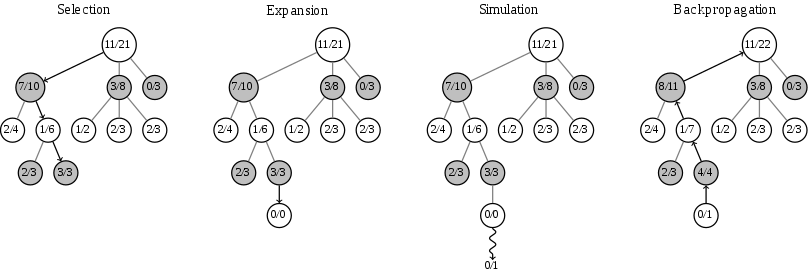
\includegraphics[width=\textwidth]{mcts}
    \caption[Diagram of general MCTS algorithm]{The 4 main parts of a rollout-based tree search. Selection: pick a child node until you get to a leaf using some criteria (UCB). Expansion: expand the leaf to include another node in your search tree, again picking the child using some criteria. Simulation: simulate the remainder of the game to get an outcome using a rollout policy. Backpropagation: update all the nodes you chose in the selection process with the new outcome.}
    \label{fig:mcts}
  \end{figure}

  Applying Monte Carlo Tree Search (MCTS) algorithms has been used to great success in many different games such as backgammon \cite{tesauro_-line_1997}, poker \cite{billings_challenge_2002}, and Scrabble \cite{sheppard_world-championship-caliber_2002}. In fact, before AlphaGo, the best Go playing program used MCTS \cite{browne_survey_2012}. It is also the underlying algorithm that powers the search in AlphaZero. However, they use a variant of the UCB for their selection process which called \textit{predictor UCB} (UCB). This variant was first proposed in \cite{rosin_multi-armed_2011} and uses a penalty term in the UCB equation to further discriminate against sufficiently bad machines. One of the main results is if you have probability distributions $P_1, \dots, P_K$ that give the exact likelihood of machine $i$ being the optimum, then one gets the following bound on regret

  \begin{gather*}
    O(\sqrt{n \log(n)} (\sum_i \sqrt{P_i})^2)
  \end{gather*}

  Thus, if we have that $P_i \sim \frac{1}{K^2}$ for most $i$, then this is an improvement over the original UCB. In the context of MCTS, this means that if we have very good estimates for the payoffs of the next nodes, and most are small, then we have a good improvement. Intuitively, this is like a human only considering bad moves (for example, moves that leave your king exposed in chess) very briefly. Finally, as we are focusing on the AlphaZero algorithm, the version of PUCT that it uses for the selection process is

  \begin{gather*}
    a_t = \argmax_{a} (Q(s_t,a) + U(s_t,a)) \text{ where } U(s,a) = c_{puct} P(s,a) \frac{\sqrt{\sum_b N(s,b)}}{1 + N(s,a)}
  \end{gather*}

  Where we are switching to the typical reinforcement learning conventions of $a_t$ designating the action, $s_t$ being the current state, $Q(s,a)$ is the value of performing action $a$ in state $s$ (you can think of this as win rate), $N(s,a)$ is the number of times action $a$ was picked in state $s$, and finally $P(s,a)$ is the prior probability of action $a$ being selected in state $s$. Notice that this scheme encourages exploration in the beginning but asymptotically prefers those with large $Q(s,a)$ values.

  \subsection{AlphaGo}

  Now that MCTS has been described, we can explain AlphaGo. At a very high level, AlphaGo is split into two parts. The first is to learn moves from a database of professional human moves. Second, it improves on this network by self play to generate new data to learn from. The first step is a supervised learning problem as you are trying to predict action probabilities from the state. That is, you are trying to find $p_{\sigma}(a | s)$ where $\sigma$ is the parameterization of the neural network. This parameterization becomes the initial network for the second step. For fast rollout procedure, a second simpler network $p_{\pi}(a | s)$ is trained.

  The second step, known as the reinforcement learning (RL) step, uses the previously trained networks to play and generate more data. The $p_{\sigma}$ network is used as the initial policy network (the one used for selecting actions in the search process) and $p_{\pi}$ is used for rollout. We call the new RL network $p_{\rho}$ that is identical in architecture as $p_{\sigma}$ and we initialize $\rho = \sigma$. A game is played and the outcome is recorded $z_t = \pm 1$, 1 for winning, and -1 for losing. The network is then updated to maximize expected outcome. That is, the change in parameters of the network follow

  \begin{gather*}
    \Delta \rho \propto \frac{\partial \log p_\rho (a_t | s_t)}{\partial \rho} z_t
  \end{gather*}

  Finally, using the self play outcomes, a value network is trained to estimate the outcome based on the current position. The network outputs a single number that tries to predict outcomes $z$ by minimizing the mean squared error between $z$ and $v_{\theta}(s)$ where $v_{\theta}$ is the neural network parameterized by $\theta$. To reduce the correlation between moves, AlphaGo was trained by playing 30 million games and picking one state-outcome pair from each game.

  With the preceding networks explained, we can now describe the MCTS regime used by AlphaGo. Recall that there four main steps: selection, expansion, simulation, backpropagation. Let us describe those four steps.

  \begin{itemize}
    \item Selection: AlphaGo uses the variant of PUCT shown above for selection. Which is shown below for convenience

    \begin{gather*}
      a_t = \argmax_{a} (Q(s_t,a) + U(s_t,a)) \text{ where } U(s,a) = c_{puct} P(s,a) \frac{\sqrt{\sum_b N(s,b)}}{1 + N(s,a)}
    \end{gather*}

    Earlier, I said that $Q(s,a)$ could be thought of as win rate which was not entirely correct. AlphaGo uses the following definition

    \begin{gather*}
      Q(s,a) = \frac{1}{N(s,a)} \sum_{i=1}^n 1_{\{(s,a,i)\}} V(s_L^i)
    \end{gather*}

    Where we have that $N(s,a) = \sum_{i=1}^n 1_{\{(s,a,i)\}}$ is the number of times state-action pair $(s,a)$ is visited. That is, $1_{\{(s,a,i)\}}$ is an indicator of the event that $(s,a)$ was visited on the $i^{th}$ simulation. We also have that $V(s_L) = (1-\lambda) v_{\theta}(s_L) + \lambda z_L$. $s_L^i$ is the leaf node on the $i^{th}$ simulation. Thus, $Q(s,a)$ is a mixture of win rate and the evaluation of the node by the valuation network. Finally, $P(s,a)$ is the prior distribution of actions given by $P(s,a) = p_{\sigma} (a | s)$

    \item Expansion: When a node $s'$ is exceeds a threshold, $N_(s',a) > n_{thr}$, that node is expanded and added to the search tree. The prior probabilities $P(s',a)$ are cached for future simulations.

    \item Simulation: The rollout network $p_{\pi}$ is used for fast simulation to get outcomes $z_t$.

    \item Backpropagation: The statistics for all the nodes visited in the simulation are updated. The visits $N(s_t,a_t) \leftarrow N(s_t,a_t) +1$ and the outcomes $W(s_t,a_t) \leftarrow W(s_t, a_t) + z_L$.

  \end{itemize}

  For the hyperparameters mentioned above, the following values were used. $\lambda =0.5$, $n_{thr} = 40$, and $c_{puct} = 5$. This gives an overarching explanation of AlphaGo without getting into the very specific techniques they used to distribute the learning. One valid question from the explanation above is where does the policy network $p_\rho$ get used? Simply, it is used to train $v_{\theta}(s)$ which is used in the evaluation of the leaf nodes in $V(s_L)$.

  \subsection{AlphaZero}

  The main difference between AlphaGo and AlphaZero is that AlphaZero omits step one, learning from human experts, and is entirely trained from self play. Another key distinction is that the input features is solely the game board. There are no human-crafted input features that are intended to help guide the search such as the number of captured stones if action $a$ is picked. There are not even redundant planes that are used to help network training. For example, the original AlphaGo uses a plane filled with 1's as an input feature presumably to help with over-fitting. In fact, AlphaGo uses 50 input planes as opposed to AlphaZero's 17. These 17 planes are the last 8 board states. Each one consisting of 2 planes, one for white stones and another for black. Finally, a $17^{th}$ plane designating which player it is.

  In many ways, the technical implementation of AlphaZero is much simpler. First of all, there is only one neural network as opposed to one for the policy and one for the value. The new network parameterized by $\theta$ tries to estimate both from the search probabilities and outcomes. That is $(p, v) = f_{\theta}(s)$ where the loss is defined to be

  \begin{gather*}
    \ell = (z-v)^2 - \pi^T \log p + c \lVert \theta \rVert^2
  \end{gather*}

  That is, it is a combination of mean-squared error between $z$ and $v$, the cross-entropy loss between $\pi$ and $p$, and an L2 regularizer. Here, $z$ are the actual outcomes of the MCTS search and $\pi$ is the empirical search probabilities. Now, one just needs to generate the training data from self play. This is done by using the same MCTS search as AlphaGo with a few differences.

  \begin{itemize}
    \item Selection: Same as AlphaGo except that the prior probabilities are \\ $P(s,a) = (p,\cdot) = f_{\theta}(s)$. Recall, there is only one network now.

    \item Expansion: Leaf nodes are always expanded and initialized with prior probabilities using $f_{\theta}$.

    \item Simulation: No rollout is used.

    \item Backpropagation: Update the statistics for visits $N(s_t,a_t) \leftarrow N(s_t,a_t) +1$ and the outcomes $W(s_t,a_t) \leftarrow W(s_t, a_t) + v$ where $v$ comes from the neural network.

  \end{itemize}

  Finally, to generate training data, once the MCTS above is performed, a move is selected using $\pi(a | s_0) = \frac{N(s_0, a)^{1/\tau}}{\sum_b N(s_0, b)^{1/\tau}}$. For the first 30 moves, $\tau = 1$ to encourage searching various openings and $\tau \rightarrow 0$ an infinitesimal is used after 30 moves to encourage only the best moves. For added exploration, the root node probabilities are subject to Dirichlet noise. That is, $P(s_0, a) = (1-\epsilon) p + \epsilon \eta$ where $\eta \sim \text{Dir}(0.03)$ and $\epsilon = 0.25$.

  Putting this all together for AlphaGo Zero. Initialize the neural network $\theta_0$ to random and denote $\alpha_{\theta_*} = \alpha_{\theta_0}$ as the best player. This notation means the tree search used by $\alpha_{\theta_i}$ uses neural network $f_{\theta_i}$. Now, $\alpha_{\theta_*}$ plays 25,000 games against itself using 1,600 MCTS iterations to select each move. For each move, record $(\pi_t, z_t)$. After those 25,000 games, train a new network $f_{\theta_{i}}$ using the loss function described earlier with these new data points from self play using moves sampled from the last 500,000 games. That is, from the last 20 self play sessions. Then, the new neural network plays 400 games against the current best network $\alpha_{\theta_*}$. If the new network wins 55\% of the games, then $f_{\theta_*} = f_{\theta_i}$. In fact, all three steps are done simultaneously: self play, training network $\theta_i$, and evaluating the best player. For AlphaZero, the one most recently published, the evaluation of the best player is omitted and a single network is continuously updated. This further simplifies the algorithm.

  \clearpage

  \section{Current Work}

  \subsection{Motivation}

  Now that the AlphaZero algorithm has been described, I can talk about what I think is its main deficiency. The deficiency is the requirement to maintain a prior probability in the PUCT. While the theory is perfectly valid for using PUCT, the requirement of maintaining a vector of length $\lvert \mathcal{A} \rvert$, the size of the action space, is onerous for the vast majority of games. For Go, there is only 361 ($19 \times 19$) possible positions to place a stone. For chess, AlphaZero cleverly represented the action policy as a fixed size of $8 \times 8 \times 73$. Consider a move as picking a square and then picking a second square to move the piece. The first part is where the $8 \times 8$ comes from. Now, suppose that you had a ``super piece'' that is a combination of every piece. That super piece could move 56 different squares as a queen (up to 7 squares in 8 directions), 8 different locations as a knight, or 9 different promotions as a pawn (default promotion is queen and therefor does not need to be specified). Imagine there to be 64 planes with a vector of length 73 each representing one possible move of the hypothetical superpiece. Note, this is slightly better than parameterizing all possible moves as picking a square and dropping it somewhere else on the board. Naively, this would yield a policy of size $64 \times 63$. However, all the promotions need to be taken into account which would turn that figure into $64 \times (63 + 3 \times 8)$ which is larger than AlphaZero's parameterization. Figure \ref{fig:chess} shows an example.

  \begin{figure}[H]
    \begin{subfigure}[h]{0.48\linewidth}
      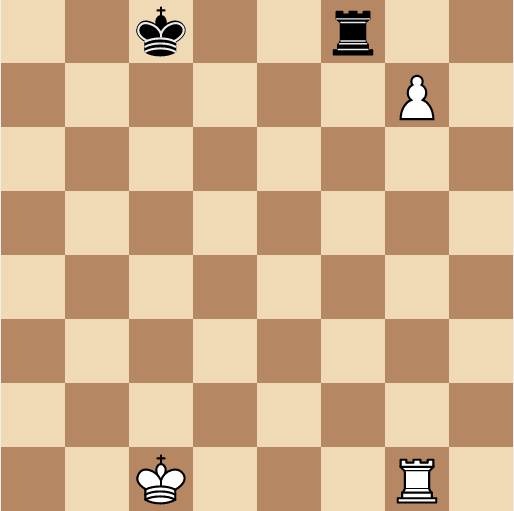
\includegraphics[width=\linewidth]{board}
      \caption{Board State}
    \end{subfigure}
    \hfill
    \begin{subfigure}[h]{0.48\linewidth}
      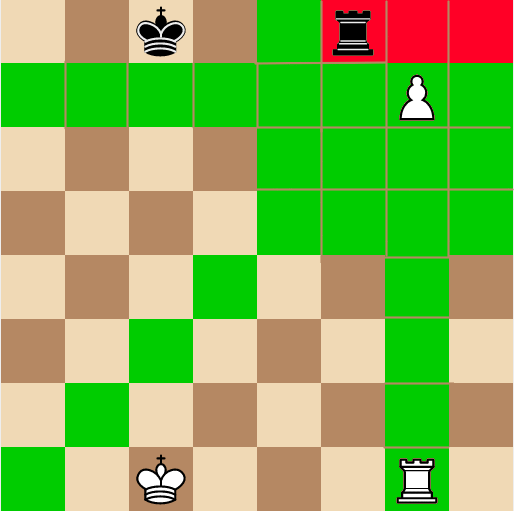
\includegraphics[width=\linewidth]{possible-moves}
      \caption{Possible Moves}
    \end{subfigure}%
    \caption[Example of chess action vector]{(a) is the current board state and (b) represents one of planes in the action vector. As the pawn is on the $49^{th}$ square, this corresponds to the $49^{th}$ plane. The green squares represents the action space and the red squares represent the 4 different promotions (bishop, knight, rook, and queen). Notice that this is only 37 actions. The other 36 fall off the board (e.g. move pawn up 2 squares).}
    \label{fig:chess}
  \end{figure}

  For completeness, the actions in the game of shogi can be completely described by fixed vector of length 11,259. Thus, the action spaces for the three different games are on the order of thousands or tens of thousands. This is after nontrivial parameterizations of the action policies. Thus, the action spaces suitable for AlphaZero must be relatively small. This presents a problem for many different games. First, AlphaZero could not be implemented for playing many strategy video games such as \textit{Starcraft} because the action space would be at least the size of a standard computer screen ($1920 \times 1080$) designating where to click next. One could attempt to compress the action space by down sampling the size of the screen, but this would fundamentally alter the what are viable actions. Without even venturing into the realm of video games, AlphaZero fails to even work for games that have previously been solved. For example, take the Scrabble AI presented in \cite{sheppard_world-championship-caliber_2002}, this is an MCTS based algorithm that has superhuman performance. It begs the question why can AlphaZero decisively beat other MCTS based algorithms in some games but not even be realistically implemented for others? Again, it ultimately comes back to having to train the network on the prior distribution. Let's examine why this is not feasible in Scrabble.

  Scrabble is a word game where the players take turns writing words on the board using the seven tiles in their possession. According to the letters they played, and any multipliers they played on, their word is scored. They then replace the letters they played from the remaining unused tiles randomly. The player with the highest score at the end of the game wins. For complete rules see \url{https://scrabble.hasbro.com/en-us/rules}. Figure \ref{fig:scrabble} shows a typical setup for the game.

  \begin{figure}[H]
    \centering
      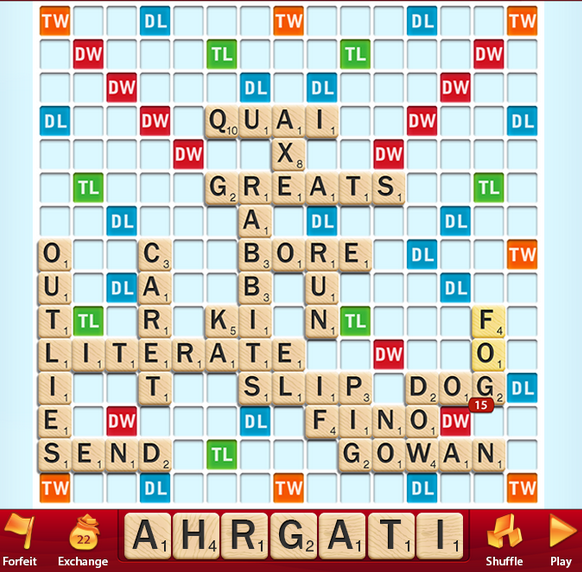
\includegraphics[width=0.5\textwidth]{scrabble}
    \caption[Example Scrabble board]{Player with the seven tiles ``AHRGATI''. Notice their opponent just played ``FO'' to spell ``FOG'' which is scored $4 \times 3 + 1 + 2$ because the F (worth 4 points) is on a triple letter.}
    \label{fig:scrabble}
  \end{figure}

  The reason why the action space for Scrabble is massive due to the sheer combination of words that can be written. According to \cite{sheppard_world-championship-caliber_2002} there are on the order of 100,000 possible English words to write. This, coupled with the fact that the board is $15 \times 15$ lower bounds the possible ways to write words at $8 \times 8 \times 100,000$ which is on the order of $10^7$, significantly larger than even the action space used for shogi. However, on any given turn, a player usually has only around 700 possible moves to make. Thus, the action space is very sparse.

  Another interesting aspect of the game of Scrabble is that of stochasticity. When tiles are played, they are replaced randomly from the underplayed tiles. As there are 100 tiles in the bag, if you played all seven of your tiles on the initial move, the number of unique racks (seven letter combinations) you can receive is enormous. This makes MCTS at anything other than small depths infeasible. Finally, the superhuman algorithms we have for playing Scrabble rely extensively on heuristics. This means that no algorithm has truly learned how to play Scrabble and simply relies on human knowledge and computational power.

  To give you an example of something one would hope a reinforcement algorithm would learn, let me give one example of the heuristics used. Rack evaluation is a heuristic that was implemented because expert human players use it as part of their strategy. The main idea is to penalize moves that leave bad letters in your rack. For example, say you have the rack ``QUIETSI'', playing the word ``SUITE'' is much worse than playing the word ``SITE''. This is because the point difference between them is 1 (a U is worth one point) but having a Q in your rack without a U is very detrimental as most words with Q are followed by the letter U. Thus, a forward looking player opts to keep Q and U together. As Scrabble AI's use a heuristic to mimic this strategy, it provides a novel opportunity to use reinforcement learning techniques to develop algorithms that extract this behavior by way of learning.

  To summarize, the game of Scrabble presents several unique research opportunities. The first being a stepping stone from games like Go and chess to a game like \textit{Starcraft} which is considered the next challenge for AI. Scrabble is in between the two in terms of the size of the action space. Second, AlphaZero has yet to be implemented on games with stochasticity. Lastly, Scrabble already has superhuman algorithms but none of these come from pure learning algorithms. Being able to beat these algorithms is a step forward for reinforcement learning.


  \subsection{Progress}

  I wish to be able to relax the AlphaZero algorithm from the necessity of the potentially large prior probability vector for the actions. That is, we wish to change the neural network from being $(p,v) = f_{\theta}(s)$ to simply $v = f_{\theta}(s)$. We know from \cite{rosin_multi-armed_2011} that we should experience a slow down of a factor of at most $\sqrt{K}$. However, there are some possibilities to reduce computation time. First, we can follow the ideas presented in \cite{bjarnason_lower_2009} and make use of Sparse UCT to improve rollout times. However, the idea that I wish to experiment with is that of inducing a prior distribution based on the values of the nodes. Doing something similar to Exploration-Exploitation with Exponential weights (EXP3) as described in \cite{audibert_minimax_2009}. However, before I can test out these ideas, I had to first build an MCTS framework that allows me to iterate quickly and modify different components in a modular way.

  What follows is the architecture of the framework that I have currently implemented. The framework follows a consumer-producer model. Where there are several types of consumers (what I will call workers) that receive tasks from a central producer (referred to henceforth as server). Figure \ref{fig:architecture} shows the architecture.

  \begin{figure}[H]
    \centering
      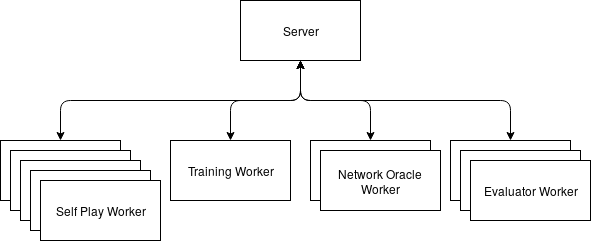
\includegraphics[width=\textwidth]{architecture}
    \caption[Architecture of framework]{Architecture of the framework.}
    \label{fig:architecture}
  \end{figure}

  This architecture was chosen because of the three different stages of AlphaZero that occur asynchronously: self-play, network training, and network evaluation. The first worker, the self play worker, simply plays games against itself using the parameters described previously. Because each game is independent, it is easily parallelized and thus you can have many self play games occuring at once. This is very important as the number of games that are required to train can exceed over a million. Once a worker is done playing a game, the result is reported to the server that keeps the history of the games. The second worker, the training worker, simply continuously trains the neural network and fetches the batches of games from the server. After 10 iterations of backpropagation, the network weights are reported to the server. It is reported to the server so that the network oracle workers can update their weights. The network oracle worker provides a nice performance boost as it removes the need of the self play workers to maintain a copy of the network and allows many workers to batch their requests to the network oracle which is much more efficient than getting the network output one at a time. Finally, the evaluator workers are optional if you wish to have more of a AlphaGo Zero type algorithm or to do ELO evaluation as part of the training process. For completeness, this architecture is accomplished using ZeroMQ as the messenger between the server and workers. It should also be noted that this diverges from the AlphaZero architecture as they have the computing resources to have a copy of the network for each self play worker.

  Another important part of the framework is to be able to test a variety of games or environments. This lead to the \textit{Game} class. The \textit{Game} class' primary role is to enforce all the rules of the game and to track a specific realization of it. The rules are enforced in the methods generate\_move and transition. These generate\_move method enumerates all valid actions while transition accounts for changes in the current\_state when an action is performed. The properties of the class are all self-explanatory, current\_state tracks the state of one realization of the game, outcome is specified when a winner is chosen, players keep track of which player is currently playing. Figure \ref{fig:tic-tac-toe} shows a toy implementation of the game Tic-Tac-Toe using this interface.

  \begin{figure}[H]
    \lstset{basicstyle=\tiny}
    \begin{lstlisting}[language=Python]
      class TicTacToe(Game):
        current_state = None
        outcome = None
        players = {'P1':1, 'P2':0}
        num_players = 2
        rows, cols = 3, 3

        def __init__(self):
          # first plane is P1 moves, second plane is P2 moves
          self.current_state = [[[0 for k in range(self.rows)]
                                    for j in range(self.cols)]
                                    for i in range(self.num_players)]

        def generate_moves(self):
          # return 2D array of open squares, assume all are open. 0=closed, 1=open
          moves = []

          for x in range(self.rows):
            for y in range(self.cols):
              valid = True
              for plane in self.current_state:
                if plane[y][x] == 1:
                  valid = False
                  break

              if valid:
                moves.append((x,y))

          return moves

        def transition(self, action):
          # use the proper player's plane to mark move
          # action is a tuple of the coordinate (x,y) to play
          plane_to_use = 0 if self.players['P1'] == 1 else 1
          x, y = action[0], action[1]

          plane = self.current_state[plane_to_use]
          plane[y][x] = 1

          # check winning condition
          if self.winning_condition():
            self.outcome = 'P1' if self.players['P1'] == 1 else 'P2'
            return

          self.players['P1'] = not self.players['P1']
          self.players['P2'] = not self.players['P2']

    \end{lstlisting}
    \caption[Toy implementation of the \textit{Game} class]{Toy implementation of the \textit{Game} class. For brevity, the \textit{winning\_condition} method is included in the Appendix.}
    \label{fig:tic-tac-toe}
  \end{figure}

  As can be seen by the toy example in Figure \ref{fig:tic-tac-toe}, the interface is quite modular and leaves much of the implementation details to the user. For example, the decision to return \textit{moves} in a 1D array could easily be replaced by a fixed 2D array that is $3 \times 3$ if one wants an action space to be of fixed length like in the AlphaZero algorithm. This modularity allows for the game class to dictate the conventions used in the game and leaves it up to the \textit{Algorithm} class to simply facilitate between the exchange of information to the \textit{Search} class. Furthermore, the \textit{Game} class requires no knowledge of the search algorithm. When the search wants to expand or rollout nodes, it simply calls \textit{generate\_moves} to build its tree and then uses \textit{transition} to move to new states. The search algorithm does not need the ability to undo moves as the state is cached in the nodes and this can be used to load a Game into that state.

  Finally, we have the \textit{MCTS} class. This is required to test the many different flavours of MCTS that one can incoporate into an AlphaZero-like algorithm. At the core, we implement the four main steps of an MCTS. To accomplish this, we must have the decision tree which is rooted at the current state of the game. The four main steps, selection, expansion, simulation, and backpropagation are broken apart to allow for easy modification of the search algorithm. The selection method will essentially implement the desired version of UCT or other algorithms based on the statistics contained in the nodes of the tree. The expansion method will grow the tree as desired. Simulation will perform the rollout procedure (or do nothing in the case of AlphaZero). Finally, backpropagation will update the statistics for the nodes involved in that iteration of the search. To reiterate, the properties and methods described above are not all encompassing of what is required in the \textit{Search} class. These represent only the most important pieces for conciseness and the minimum of what should be implemented for the \textit{Algorithm} class to function. For example, search hyperparameters such as expansion depth, will also need to be stored in this class but is not required to have a useful interface.

  As for my progress in developing the framework, I have fully developed the framework and have it running locally on a toy game. The toy game is the games Pawns; Chess without the backrow pieces and the goal is to be the first to advanced a pawn to the end row. At this stage, the first next step is to refactor my codebase as it is rather complicated at the moment. During the refactor, I will profile and optimize the individual workers. Next is to prepare the code and execute it on the Princeton cluster. Finally, I hope to extend to further games and environments. Table \ref{table:milestones} summarizes the short term milestones I have set for myself.

  \begin{table}[H]
    \caption{Short term milestones and my expected date of completion}
    \label{table:milestones}
    \begin{center}
      \begin{tabular}{| p{0.5\textwidth} | c |}
        \hline
        Milestone & Planned Date \\
        \hline
        Refactor and optimize & May \\
        \hline
        Framework running on cluster & June \\
        \hline
        Reproduce basic AlphaZero results & June-July \\
        \hline
        Compare with AlphaZero variations & July-August \\
        \hline
        Taking the best variations and applying them to the game of Scrabble & August \\
        \hline
        Begin writing paper with results with ICML in mind & Fall \\
        \hline
      \end{tabular}
    \end{center}
  \end{table}

  \subsection{Future Work}

  This area of research is ripe with open questions and the work presented above can go in multiple different directions both in theory and applications. I will focus on the extensions of this work to other future applications. The following discussion is contingent on the alterations I propose to AlphaZero working for games with large action spaces.

  The obvious direction to go is trying to achieve superhuman performance at \textit{Starcraft}. As outlined earlier, \textit{Starcraft} is difficult to solve both because of the large state space and action space. Using neural networks like AlphaZero gives us hope that we can tackle the state space issue. However, even using human heuristics, it would be difficult to reduce the number of actions one needs to explore. This is further exacerbated by the issue that developing complex behavior in \textit{Starcraft} often requires planning minutes ahead of time which can be on the order of 400 actions before an action's benefit is realized. Thus, to even evaluate the benefits of an action, the depth of the tree would have to be larger than that used to train AlphaZero. Without good theory and techniques to tackle this large of a problem, a simpler game should be chosen. Recently, \text{Two Sigma} developed a programming challenge to see who could develop the best program at playing a game they invented called Halite II. Figure \ref{fig:halite} shows a game of Halite II in progress.

  \begin{figure}[H]
    \centering
      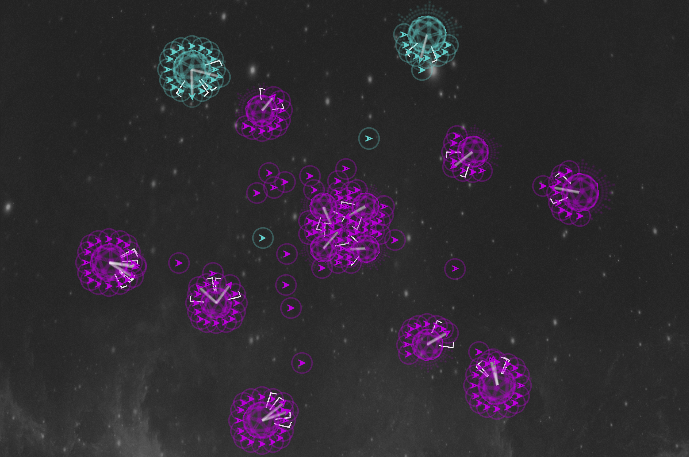
\includegraphics[width=0.7\textwidth]{halite}
    \caption[A game of Halite II in progress]{The goal of the game is to conquer planets that yields more ships and destroy your enemy's forces.}
    \label{fig:halite}
  \end{figure}

  Halite II is a great stepping stone towards \textit{Starcraft} because it requires the same type of decision making but on a much smaller scale. One, the game is realtime so your opponent does not have to wait for you. Two, it is a balance of growing one's forces and spreading to other planets while preventing your opponent from doing so. It is essentially \textit{Starcraft} but with only one type of unit and production of units being fixed to an automatic process outside of your control. It also has a large community and well established testing environment which is ideal for research.

  Another avenue to explore in the games realm is that of multiplayer games. The theory behind MCTS is supported by two player zero sum games but there is work being done to extend it to find mixed-strategies in multiplayer games \cite{sturtevant_analysis_2008}. Another interesting area of multiplayer games is whether one can alter the selection process of MCTS to better converge onto exploitative strategies based on past behavior in multiplayer games.

  Shifting the focus away from games. Alluded to throughout the previous section was the ability to apply my framework to different environments. It would be interesting to take the my framework and apply it to a robotic environment such as MuJoCo and to test the effectiveness of training robots in a simulated physics environment. It would be interesting to compare AlphaZero to other state of the art methods of training robots. Figure \ref{fig:mujoco} shows an example simulation in the MuJoCo environment.

  \begin{figure}[H]
    \centering
      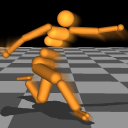
\includegraphics[width=0.5\textwidth]{mujoco}
    \caption[Sample MuJoCo Environment]{An example of one of the many different simulation environments in MuJoCo.}
    \label{fig:mujoco}
  \end{figure}

  Moving on to the more theoretical work, it would be interesting to investigate the behavior of different schemes of inducing different probability distributions over the $K$ arms of a multi-armed bandit. For example, under what assumptions of the rewards distribution does one need to have improvements under schemes like EXP3.

  In general, investigating different techniques on how to handle large state or action spaces is an intriguing area to me. Work being done in hierarchal learning using deep Q-networks shows promise in solving notoriously hard games \cite{kulkarni_hierarchical_2016}. Exploring the MAXQ algorithm developed in \cite{dietterich_hierarchical_1999} and trying to relax the necessity of the structure of the hierarchy being programmed into the learning algorithm by an expert is an exciting research direction.

  One area of recent development that is especially interesting to me is that of using MCTS for imitation learning. The recently published algorithm ExIt (Expert Iteration) is quite similar to the AlphaGo algorithm except a new policy network that imitates the best known expert is created every loop. This approach was able to beat the best known programs at the game of Hex \cite{anthony_thinking_2017}.

  \section{Conclusion}

  Throughout this report, I gave a thorough treatment to how the AlphaZero algorithm works from both a theoretical and technical implementation point of view. By dissecting the shortcomings of the algorithm, I presented some modifications to the algorithm that might be able to allow it to tackle a wider range of games. This motivated the reason why I am working on a MCTS framework to experiment with different variations with the ultimate goal of developing the best known Scrabble program. I then presented other areas of related research that might benefit from similar techniques that could be future research topics.

  \clearpage

  \bibliography{references}
  \bibliographystyle{ieeetr}

  \clearpage

  \appendix

  \section*{Appendix}

  \lstset{basicstyle=\tiny}
  \begin{lstlisting}[language=Python]
    def winning_condition(self):
      # check winning condition, rows
      for x in range(self.rows):
        count = 0
        for y in range(self.cols):
          count += plane[y][x]

        if count == 3:
          self.outcome = 'P1' if self.players['P1'] == 1 else 'P2'
          return

      # check winning condition, columns
      for y in range(self.cols):
        count = 0
        for x in range(self.rows):
          count += plane[y][x]

        if count == 3:
          self.outcome = 'P1' if self.players['P1'] == 1 else 'P2'
          return

      # check winning condition, diagonals
      count = 0
      for x in range(self.rows):
        count += plane[x][x]

      if count == 3:
        self.outcome = 'P1' if self.players['P1'] == 1 else 'P2'
        return

      count = 0
      for x in range(self.rows):
        count += plane[x][-1-x]

      if count == 3:
        self.outcome = 'P1' if self.players['P1'] == 1 else 'P2'
        return

    \end{lstlisting}

\end{document}